\documentclass{article}

\usepackage[english]{babel}
\usepackage[a4paper,top=2cm,bottom=2cm,left=3cm,right=3cm]{geometry}
\usepackage{amsmath}
\usepackage{amssymb}
\usepackage{amsthm}
\usepackage{booktabs}
\usepackage{graphicx}
\usepackage[colorlinks=true, allcolors=blue]{hyperref}

\newtheorem{theorem}{Theorem}[section]
\newtheorem{proposition}[theorem]{Proposition}
\newtheorem{definition}[theorem]{Definition}
\newtheorem{lemma}[theorem]{Lemma}
\newtheorem{corollary}[theorem]{Corollary}
\newtheorem{remark}[theorem]{Remark}
\newtheorem{question}{Question}

\title{A Euclidean View of the Non-Homomorphism Factor:\\
       the Profile of a Graph}
\author{Mohammad Ali Rostami}
\date{Draft, \today}

\begin{document}
\maketitle

\begin{abstract}
The non-homomorphism factor $|G,H|$ is the minimum number of edges that must
be deleted from $G$ so that the remaining graph admits a homomorphism to $H$.
The symmetric quantity $\max(|G,H|,|H,G|)$ is not a metric, and its
shortest-path closure is a metric that is not Euclidean.  We study instead
the \emph{profile} of a graph $G$: the vector of normalised values
$|T,G|/|E(T)|$ over a family of test graphs $T$.  The profile depends only
on the homomorphism class of $G$, reverses the homomorphism order, and yields
an exact Euclidean metric.  We give closed forms for its clique and
odd-cycle coordinates, which lead to a strengthening of the clique lower
bound for $|G,H|$.  We show that no family of bounded-size tests can detect
the chromatic number, and relate the profile to the separation parameter of
F\"arnqvist, Jonsson and Thapper and to the concentration parameter.
Computations on all $1276$ cores with at most $9$ vertices, on the
generalized Petersen graphs $GP(n,k)$ with $n\le12$, and on the circular
cliques $K_{p/q}$ with $p\le13$, illustrate the geometry of the resulting
space.
\end{abstract}

\section{Introduction}

For graphs $G$ and $H$, the \emph{non-homomorphism factor} $|G,H|$ is the
minimum number of edges whose removal from $G$ leaves a graph that maps
homomorphically to $H$~\cite{khoshkha2005}.  Deciding whether $|G,H|\le k$
is the problem \textsc{Edge Deletion-$H$-Colouring}~\cite{foucaud2019}.  It
is NP-hard whenever the core of $H$ has more than one edge, by the
Hell--Ne\v{s}et\v{r}il dichotomy~\cite{hell2004}.

A natural attempt to measure how far apart two graphs are is
$\operatorname{dist}(G,H)=\max(|G,H|,|H,G|)$.  It is symmetric and, on
cores, vanishes only on isomorphic pairs.  However, it is not a metric:
\[
  \operatorname{dist}(K_2,K_5)=4\;>\;3=\operatorname{dist}(K_2,K_3)+\operatorname{dist}(K_3,K_5).
\]
The failure is unbounded.  The chain $K_n,K_{n-1},\dots,K_2$ has total
length $n-2$, while $\operatorname{dist}(K_n,K_2)\approx n^2/4$.  The
largest metric below $\operatorname{dist}$ is its shortest-path closure
$d^*$, for which $d^*(K_n,K_m)=|n-m|$.  But $d^*$ cannot be embedded
isometrically in any Euclidean space.  Indeed, $d^*(K_3,K_4)=d^*(K_4,K_5)=d^*(K_4,I)=1$,
where $I$ is the icosahedron, while the three distances among $K_3$, $K_5$
and $I$ all equal $2$.  In a Euclidean space, $K_4$ would have to be the
midpoint of all three pairs, which is impossible.

This paper takes a different route.  Instead of comparing two graphs
directly, we describe each graph by how a fixed family of test graphs maps
\emph{into} it.  This gives the \emph{profile} of a graph, and ordinary
Euclidean distance between profiles.

Throughout, $\operatorname{mc}_G(T)=|E(T)|-|T,G|$ denotes the largest number
of edges of $T$ preserved by a vertex map $V(T)\to V(G)$.  This is the
optimum of the \textsc{Max $G$-Col} problem~\cite{fjt2009,efjt2015}, also
called maximum graph homomorphism~\cite{lrs2006}.  We write $t(n,r)$ for
the number of edges of the Tur\'an graph $T(n,r)$.

Several of the statements below are known in the language of the
\emph{separation} parameter of Engstr\"om, F\"arnqvist, Jonsson and
Thapper~\cite{efjt2015}; we indicate this where it applies.  What we add is
the Euclidean embedding, the improved lower bound
(Remark~\ref{rem:omega_bound}), the blindness result
(Proposition~\ref{prop:profile_blind}), the link to the concentration
parameter (Proposition~\ref{prop:profile_lip}), and the computations of
Section~\ref{sec:computations}.

% ---------------------------------------------------------------------------
\section{The profile and the profile metric}
\label{sec:profile}

\begin{definition}[Profile]
\label{def:profile}
Let $\mathfrak F$ be a countable family of graphs, each with at least one
edge (the \emph{test graphs}).  For a graph $G$ with at least one edge, the
\emph{profile} of $G$ is
\[
  \varphi(G)=\bigl(\varphi_T(G)\bigr)_{T\in\mathfrak F},\qquad
  \varphi_T(G)=\frac{|T,G|}{|E(T)|}\in[0,1].
\]
Given weights $w\colon\mathfrak F\to(0,\infty)$ with
$\sum_T w_T<\infty$, the \emph{profile distances} are
\[
  E_w(G,H)=\Bigl(\sum_{T\in\mathfrak F}w_T\bigl(\varphi_T(G)-\varphi_T(H)\bigr)^2\Bigr)^{1/2},
  \qquad
  E_\infty(G,H)=\sup_{T\in\mathfrak F}\bigl|\varphi_T(G)-\varphi_T(H)\bigr|.
\]
\end{definition}

$E_w$ is the distance of the Hilbert space $\ell^2(\mathfrak F,w)$
restricted to the set of profiles, so it is Euclidean by construction.
The profile is the target-side, max-plus analogue of Lov\'asz's vector
of homomorphism numbers $(\hom(T,G))_T$~\cite{lovasz1967,dgr2018}.  Its zero
set $\{T:\varphi_T(G)=0\}=\{T: T\to G\}$ is the qualitative version of that
vector.  Unlike the source-side quantity $|G,H|$, the profile depends only on
the homomorphism class of $G$.  For example, $|2K_4,K_3|=2\neq1=|K_4,K_3|$,
although $2K_4$ and $K_4$ are homomorphically equivalent.

\begin{proposition}[Monotonicity and order embedding]
\label{prop:profile_order}
\begin{enumerate}
\item[(a)] If $G\to H$, then $\varphi_T(G)\ge\varphi_T(H)$ for every $T$.
      In particular, $\varphi(G)=\varphi(H)$ whenever $G$ and $H$ are
      homomorphically equivalent.
\item[(b)] If $\mathfrak F$ contains a graph homomorphically equivalent to
      $G$, then $\varphi(G)\ge\varphi(H)$ implies $G\to H$.
\end{enumerate}
Consequently, if $\mathfrak F$ contains all connected cores, then
$G\mapsto\varphi(G)$ is an order-reversing embedding of the homomorphism
order of connected graphs into $([0,1]^{\mathfrak F},\le)$.  In that case
$E_w$ and $E_\infty$ are metrics on homomorphism classes, and for finite
$\mathfrak F$ the sum $\|\varphi(G)\|_1$ is a strictly decreasing height
function on the cores in $\mathfrak F$.
\end{proposition}

\begin{proof}
(a) If $T-S\to G\to H$, then $T-S\to H$.  This is the profile form
of~\cite[Lemma~2.6]{efjt2015}.
(b) Let $T\in\mathfrak F$ with $T\leftrightarrow G$.  Then
$0=\varphi_T(G)\ge\varphi_T(H)$, so $G\to T\to H$.
\end{proof}

Part (b) needs a graph equivalent to $G$ itself; a graph equivalent to $H$
is not enough.  For example, with $\mathfrak F=\{K_2\}$ we have
$\varphi_{K_2}(K_3)=0=\varphi_{K_2}(K_2)$, so $\varphi(K_3)\ge\varphi(K_2)$,
although $K_3\not\to K_2$.

The embedding is not a lattice map.  The join and meet of the homomorphism
order are $G\sqcup H$ and $G\times H$.  They satisfy
$\varphi(G\sqcup H)\le\min(\varphi(G),\varphi(H))$ and
$\varphi(G\times H)\ge\max(\varphi(G),\varphi(H))$, and both inequalities
can be strict.  For example, let $T$ be $K_3$ and the Gr\"otzsch graph
$\mathrm{Gr}$ joined by a bridge.  Then $|T,K_3|=|T,\mathrm{Gr}|=1$, but
$|T,K_3\times\mathrm{Gr}|=2$.

% ---------------------------------------------------------------------------
\section{Closed forms and what the profile can read}

\begin{proposition}[Clique and odd-cycle coordinates]
\label{prop:profile_closed}
Let $G$ have $\omega(G)=r\ge2$ and odd girth $g$, with $g=\infty$ if $G$ is
bipartite.  For every $n\ge2$ and $k\ge1$,
\[
  |K_n,G|=\binom n2-t\bigl(n,\min(n,r)\bigr),\qquad
  \varphi_{C_{2k+1}}(G)=
  \begin{cases}0,&2k+1\ge g,\\[2pt] \dfrac1{2k+1},&2k+1<g.\end{cases}
\]
Every bipartite test has $\varphi_T(G)=0$.  Hence $\omega(G)$ and the odd
girth of $G$ can be read off $\varphi(G)$:
$\omega(G)\ge n\iff\varphi_{K_n}(G)=0$, and
$g\le 2k+1\iff\varphi_{C_{2k+1}}(G)=0$.
\end{proposition}

\begin{proof}
The preserved edges of $K_n$ form a graph that maps to $G$.  Cliques map
injectively, so this graph is $K_{r+1}$-free, and by Tur\'an's theorem it
has at most $t(n,r)$ edges.  Mapping $K_n$ in a balanced way onto an
$r$-clique of $G$ attains this bound.  For odd cycles, $C_{2k+1}\to G$ if
and only if $G$ has an odd cycle of length at most $2k+1$.  Otherwise,
deleting one edge leaves a path, which maps to an edge.  In the language of
separation these are~\cite[Props.~2.4, 2.5]{efjt2015}.
\end{proof}

\begin{remark}[An $\omega$-version of the clique lower bound]
\label{rem:omega_bound}
The same argument gives, for all graphs $G$ and $H$,
\[
  |G,H|\ \ge\ |E(G)|-t\bigl(|V(G)|,\omega(H)\bigr),
\]
because every subgraph of $G$ that maps to $H$ is $K_{\omega(H)+1}$-free.
Since $\omega(H)\le\chi(H)$, this is never weaker than the bound
$|G,H|\ge|E(G)|-t(|V(G)|,\chi(H))$, and it is attained by $G=K_n$ for
\emph{every} $H$.  For example, $|K_5,C_5|=4$: the largest triangle-free
subgraph of $K_5$ is $K_{2,3}$, which maps to $C_5$.  The $\chi$-bound gives
only $10-t(5,3)=2$.
\end{remark}

\begin{proposition}[Range of the profile]
\label{prop:profile_range}
For every $G$ with an edge and every test $T$,
$\varphi_T(G)\le\varphi_T(K_{\omega(G)})\le 1/\omega(G)$.
Moreover, $\varphi_{K_n}(G)\to1/\omega(G)$ as $n\to\infty$, so
$\sup_T\varphi_T(G)=1/\omega(G)$.  In particular,
$E_\infty(G,H)\ge\bigl|1/\omega(G)-1/\omega(H)\bigr|$ when $\mathfrak F$
contains all complete graphs.
\end{proposition}

\begin{proof}
The first inequality is Proposition~\ref{prop:profile_order}(a) applied to
$K_{\omega(G)}\to G$.  For the second, colour $V(T)$ uniformly at random
with $\omega(G)$ colours.  Each edge is properly coloured with probability
$1-1/\omega(G)$, so some colouring preserves at least that fraction of
$E(T)$.  The limit follows from Proposition~\ref{prop:profile_closed}.
\end{proof}

\begin{proposition}[Bounded tests cannot see $\chi$]
\label{prop:profile_blind}
Suppose every $T\in\mathfrak F$ has at most $m$ vertices, and $G$ has an
edge and odd girth larger than $m$.  Then $\varphi(G)=\varphi(K_2)$ on
$\mathfrak F$.
\end{proposition}

\begin{proof}
Let $f\colon V(T)\to V(G)$.  The image of the preserved edges is a subgraph
of $G$ on at most $m$ vertices.  It has no odd cycle, so it maps to an edge
of $G$.  Hence $\operatorname{mc}_G(T)=\operatorname{mc}_{K_2}(T)$.
\end{proof}

By Erd\H{o}s' theorem on graphs of large girth and large chromatic
number~\cite{erdos1959}, no finite family of tests detects $\chi$, the
fractional chromatic number, or even bipartiteness.  With summable weights,
$E_w(G,K_2)\to0$ along any sequence of graphs whose odd girth tends to
infinity, whatever their chromatic numbers.  Concretely, the generalized
Mycielskian $\mu_5(C_{11})$ ($67$ vertices, $\chi=4$) has the same profile
as $K_2$ on the twelve tests $K_2,\dots,K_6$, $C_5$, $C_7$, $C_9$, Petersen,
Gr\"otzsch, $W_5$ and the icosahedron.  Section~\ref{sec:computations}
shows the same effect on generalized Petersen graphs.

Circular cliques show the mechanism precisely.  Recall that $K_{p/q}$
($\gcd(p,q)=1$, $p\ge2q$) has vertex set $\mathbb Z_p$, with $i\sim j$ if
and only if $q\le|i-j|\le p-q$; then $K_{n/1}=K_n$ and
$K_{(2k+1)/k}=C_{2k+1}$.  A graph $X$ with an edge maps to $K_{p/q}$ if and
only if its circular chromatic number satisfies $\chi_c(X)\le p/q$, and
$\chi_c(X)=a/b$ for some $a\le|V(X)|$~\cite{vince1988,zhu2001}.  For a
rational $r\ge2$, let $\lfloor r\rfloor_m$ be the largest fraction $a/b\le r$
with $a\le m$.

\begin{proposition}[Farey staircase]
\label{prop:circular}
If every $T\in\mathfrak F$ has at most $m$ vertices, then
$\varphi(K_{p/q})=\varphi\bigl(K_{\lfloor p/q\rfloor_m}\bigr)$ on $\mathfrak F$.
\end{proposition}

\begin{proof}
Let $T\in\mathfrak F$ and $S\subseteq E(T)$.  The graph $T-S$ has at most
$m$ vertices, so $\chi_c(T-S)$ is a fraction with numerator at most $m$.
Hence $\chi_c(T-S)\le p/q$ if and only if
$\chi_c(T-S)\le\lfloor p/q\rfloor_m$, that is, $T-S\to K_{p/q}$ if and only
if $T-S\to K_{\lfloor p/q\rfloor_m}$.  So $|T,K_{p/q}|=|T,K_{\lfloor p/q\rfloor_m}|$.
\end{proof}

Proposition~\ref{prop:profile_blind} restricted to odd cycles is the case
$\lfloor (2k+1)/k\rfloor_m=2$ for $2k+1>m$.  Along the chain of circular
cliques, which is a chain in the homomorphism order, the profile is
therefore a staircase: it only moves at fractions with small numerators.

% ---------------------------------------------------------------------------
\section{The source-side profile}

The profile records what maps \emph{into} $G$.  The chromatic number is a
statement about where $G$ maps \emph{to}, so it calls for the dual object.
The naive candidate $|G,T|/|E(G)|$ is not constant on homomorphism classes,
so we use weights.

\begin{definition}
For a graph $G$ with an edge and a test $T$, let
\[
  \psi_T(G)=\max_{w}\ \frac{|G,T|_w}{\|w\|_1},
\]
where the maximum is over non-negative, non-zero edge weights $w$ on $G$,
and $|G,T|_w$ is the minimum total weight of edges whose deletion leaves a
graph mapping to $T$.
\end{definition}

\begin{proposition}
\label{prop:psi}
$\psi_T(G)=1-s(T,G)$, where $s$ is the separation of
F\"arnqvist, Jonsson and Thapper~\cite{fjt2009,efjt2015}.  Moreover:
\begin{enumerate}
\item[(a)] $\psi_T$ is constant on homomorphism classes and order-preserving:
           $G\to H$ implies $\psi_T(G)\le\psi_T(H)$.
\item[(b)] $\psi_T(G)=0$ if and only if $G\to T$.  In particular
           $\psi_{K_k}(G)>0$ if and only if $\chi(G)>k$.
\item[(c)] $\psi(G\sqcup H)=\max(\psi(G),\psi(H))$ and
           $\psi(G\times H)\le\min(\psi(G),\psi(H))$.
\item[(d)] $|G,T|/|E(G)|\le\psi_T(G)$, with equality if $G$ is edge-transitive.
\end{enumerate}
\end{proposition}

\begin{proof}[Sketch]
The identity with $1-s(T,G)$ is~\cite[Thm.~2.1, Cor.~2.11]{efjt2015}, which
also shows the maximum is attained by automorphism-invariant weights on $G$
itself.  By~\cite[Prop.~5.4]{efjt2015} it equals $1-1/\chi_T(G)$, where
$\chi_T$ is the fractional covering number by $T$-cuts; for $T=K_2$ this is
\v{S}\'amal's cubical chromatic number~\cite{samal2015}.  (a)--(c) follow
from the definition, and (d) from averaging over automorphisms.
\end{proof}

Thus $\varphi$ reads the clique number and $\psi$ reads the chromatic
number.  The gap $\chi-\omega$ appears as the distance between the two
readings; see Figure~\ref{fig:final}(b).  Hedetniemi's conjecture asserted
that $\chi(G\times H)>k$ whenever $\chi(G)>k$ and $\chi(H)>k$.  In profile
terms, it asserted that $\psi_{K_k}(G)>0$ and $\psi_{K_k}(H)>0$ imply
$\psi_{K_k}(G\times H)>0$.  Shitov's counterexamples~\cite{shitov2019}
show that this fails, so by Proposition~\ref{prop:psi}(c) the inequality
$\psi(G\times H)\le\min(\psi(G),\psi(H))$ can be strict even on the
support.

% ---------------------------------------------------------------------------
\section{Three distances on one embedding}

\begin{proposition}[Relation to separation]
\label{prop:profile_fjt}
For edge-weighted graphs $(T,w)$, write
$p_G(T,w)=\operatorname{mc}_G(T,w)/\|w\|_1$; for unit weights,
$p_G(T)=1-\varphi_T(G)$.  The separation of~\cite{fjt2009,efjt2015} is
$s(G,H)=\inf_{(T,w)}p_G(T,w)/p_H(T,w)$.
\begin{enumerate}
\item[(a)] If $T$ is edge-transitive, then $\varphi_T(G)=1-s(G,T)$
      \cite[Thm.~2.1]{efjt2015}.
\item[(b)] The additive form of the FJT metric is the Hilbert projective
      metric on profiles:
      \[
        -\log s(G,H)-\log s(H,G)
        =\log\sup_{(T,w)}\frac{p_H(T,w)}{p_G(T,w)}
        +\log\sup_{(T,w)}\frac{p_G(T,w)}{p_H(T,w)},
      \]
      and the FJT distance is $d_{\mathrm{FJT}}=1-s(G,H)s(H,G)=1-e^{-d_{\mathrm{Hilb}}}$.
      For a finite unweighted family $\mathfrak F$, the same expression with
      the suprema over $T\in\mathfrak F$ is a pseudometric.  It is a metric
      on the homomorphism classes of graphs whose cores lie in $\mathfrak F$.
\end{enumerate}
\end{proposition}

\begin{proof}
(a) is the edge-transitive case of \cite[Thm.~2.1]{efjt2015}.  (b) is the
definition of $s$, rewritten.  Positivity on a finite family follows as in
Proposition~\ref{prop:profile_order}(b).
\end{proof}

So the sup-distance $E_\infty$, the Euclidean distance $E_w$ and the FJT
metric are three distances on one embedding $G\mapsto\varphi(G)$.  Only the
FJT metric carries an approximation-theoretic meaning~\cite[Lemma~1.6]{efjt2015};
only $E_w$ is Euclidean.

\begin{proposition}[Moving the target; link to concentration]
\label{prop:profile_lip}
Let $S\subseteq E(T)$ with $|S|=|T,G|$, and let $f\colon T-S\to G$ be a
homomorphism.  Let $\mu(f)$ be the largest number of edges of $T-S$ that
$f$ maps onto a single edge of $G$.  For every graph $H$,
\[
  |T,H|\ \le\ |T,G|+\mu(f)\,|G,H|.
\]
In particular, if $T\to G$, then $|T,H|\le\gamma(T,G)\,|G,H|$, where
$\gamma$ is the concentration parameter.  Also $|T,G-e|\le|T,G|+\mu(f,e)$
for every $e\in E(G)$, where $\mu(f,e)$ is the load of $e$.
\end{proposition}

\begin{proof}
Let $S'\subseteq E(G)$ be optimal with $g\colon G-S'\to H$.  Delete from
$T-S$ the at most $\mu(f)|S'|$ edges that $f$ maps into $S'$.  The map
$g\circ f$ is then a homomorphism from what remains to $H$.
\end{proof}

The same inequality, with $T$ replaced by $G$, is what breaks the triangle
inequality for $\operatorname{dist}$: the composition cost is multiplied by
the load.  The concentration parameter is therefore the local Lipschitz
constant of the profile under changes of the target.  The jump can be large:
deleting a triangle edge from $K_3$ with a long pendant path changes
$\varphi_{K_3}$ from $0$ to $1/3$, however many edges the graph has.

\begin{remark}[Computation]
We have
\[
  \operatorname{mc}_G(T)=\lim_{\beta\to\infty}\beta^{-1}\log\hom(T,W_\beta),
\]
where $W_\beta$ is the looped complete graph on $V(G)$ with weight $e^\beta$
on $E(G)$ and $1$ elsewhere.  Consequently, the tree-decomposition dynamic
program for $\hom(T,\cdot)$, run over the $(\max,+)$ semiring, computes
$\varphi_T(G)$ in time
$O\bigl(|V(T)|\,|V(G)|^{\operatorname{tw}(T)+1}\bigr)$.
\end{remark}

% ---------------------------------------------------------------------------
\section{Computations}
\label{sec:computations}

\paragraph{Data.}
All values below are exact.  We computed $|T,G|$ for all pairs among the
$1276$ cores of connected graphs on at most $9$ vertices (plus a few named
graphs), with a branch-and-bound solver.  The default test family is the
set of $85$ cores consisting of all cores on at most $8$ vertices together
with $C_9$, $C_{11}$, the Petersen graph, the Gr\"otzsch graph and the
icosahedron.  Each test $T$ receives the weight $w_T=1/\sqrt{N_{\chi(T)}}$,
where $N_c$ is the number of tests with chromatic number $c$, so that each
chromatic class of tests carries the same total squared weight.  With
these weights $E_w$ correlates $0.92$ with $\operatorname{dist}$ and $0.83$
with $d^*$ (Pearson), better than with uniform weights ($0.78$ and $0.59$).
Removing any single test changes the ranking of distances very little
(Spearman $\rho\ge0.9995$).

\paragraph{Geometry.}
Figure~\ref{fig:pca} shows the first two principal components.  The first
axis carries $92\%$ of the variance and is, up to sign, the height
$\|\varphi\|_1$ of Proposition~\ref{prop:profile_order}.  Along the
$615{,}167$ comparable pairs $G\to H$ among the $1276$ cores it never
decreases.  The complete graphs form a chain $K_8,K_7,\dots,K_3$ that then
jumps to $K_2$ at the triangle-free end, where the odd cycles accumulate:
$C_{2k+1}\to K_2$ in the profile metric, as
Proposition~\ref{prop:profile_closed} predicts.  Nearest neighbours share
the clique number in $96\%$ of cases but the chromatic number in only
$81\%$; this agrees with Proposition~\ref{prop:profile_closed} and
Proposition~\ref{prop:profile_blind}.

\paragraph{Generalized Petersen graphs.}
We computed the full $85$-test profile of all $30$ graphs $GP(n,k)$ with
$3\le n\le 12$ and $1\le k<n/2$ (Table~\ref{tab:gp}).  Every one of them
lands \emph{exactly} on the profile of one of the seven cores $K_2$, $K_3$,
$C_5$, $C_7$, $C_9$, $C_{11}$ or Petersen.  For $19$ of them, including
$GP(5,2)$, which is the Petersen graph itself, this is because they are
homomorphically equivalent to that core.  The other $11$ are $3$-chromatic
graphs of odd girth $5$ or $7$ that do \emph{not}
map to $C_5$ or $C_7$, as an exhaustive search confirms.  Yet no test with
at most $12$ vertices distinguishes them from the cycle.  The dodecahedron
$GP(10,2)$ is such a graph.

\begin{table}[ht]
\centering
\small
\begin{tabular}{@{}p{2.3cm}p{5.2cm}p{5.2cm}@{}}
\toprule
Profile equals that of & Homomorphically equivalent & Same profile, \emph{not} equivalent \\
\midrule
$K_2$ & $GP(4,1)$, $GP(6,1)$, $GP(8,1)$, $GP(8,3)$, $GP(10,1)$, $GP(10,3)$, $GP(12,1)$, $GP(12,3)$, $GP(12,5)$ & --- \\
$K_3$ & $GP(3,1)$, $GP(6,2)$, $GP(9,3)$, $GP(12,4)$ & --- \\
$C_5$ & $GP(5,1)$, $GP(10,4)$ & $GP(7,2)$, $GP(7,3)$, $GP(8,2)$, $GP(9,2)$, $GP(9,4)$, $GP(10,2)$, $GP(11,2)$, $GP(11,5)$, $GP(12,2)$ \\
$C_7$ & $GP(7,1)$ & $GP(11,3)$, $GP(11,4)$ \\
$C_9$ & $GP(9,1)$ & --- \\
$C_{11}$ & $GP(11,1)$ & --- \\
Petersen & $GP(5,2)$ & --- \\
\bottomrule
\end{tabular}
\caption{Where the generalized Petersen graphs $GP(n,k)$, $3\le n\le12$,
land in the profile space of the $85$ test cores.  The left column lists
graphs that are homomorphically equivalent to the core (bipartite, or
containing a triangle, or mapping onto their shortest odd cycle).  The
right column lists graphs with exactly the same profile but no
homomorphism to the cycle.}
\label{tab:gp}
\end{table}

\begin{figure}[ht]
\centering
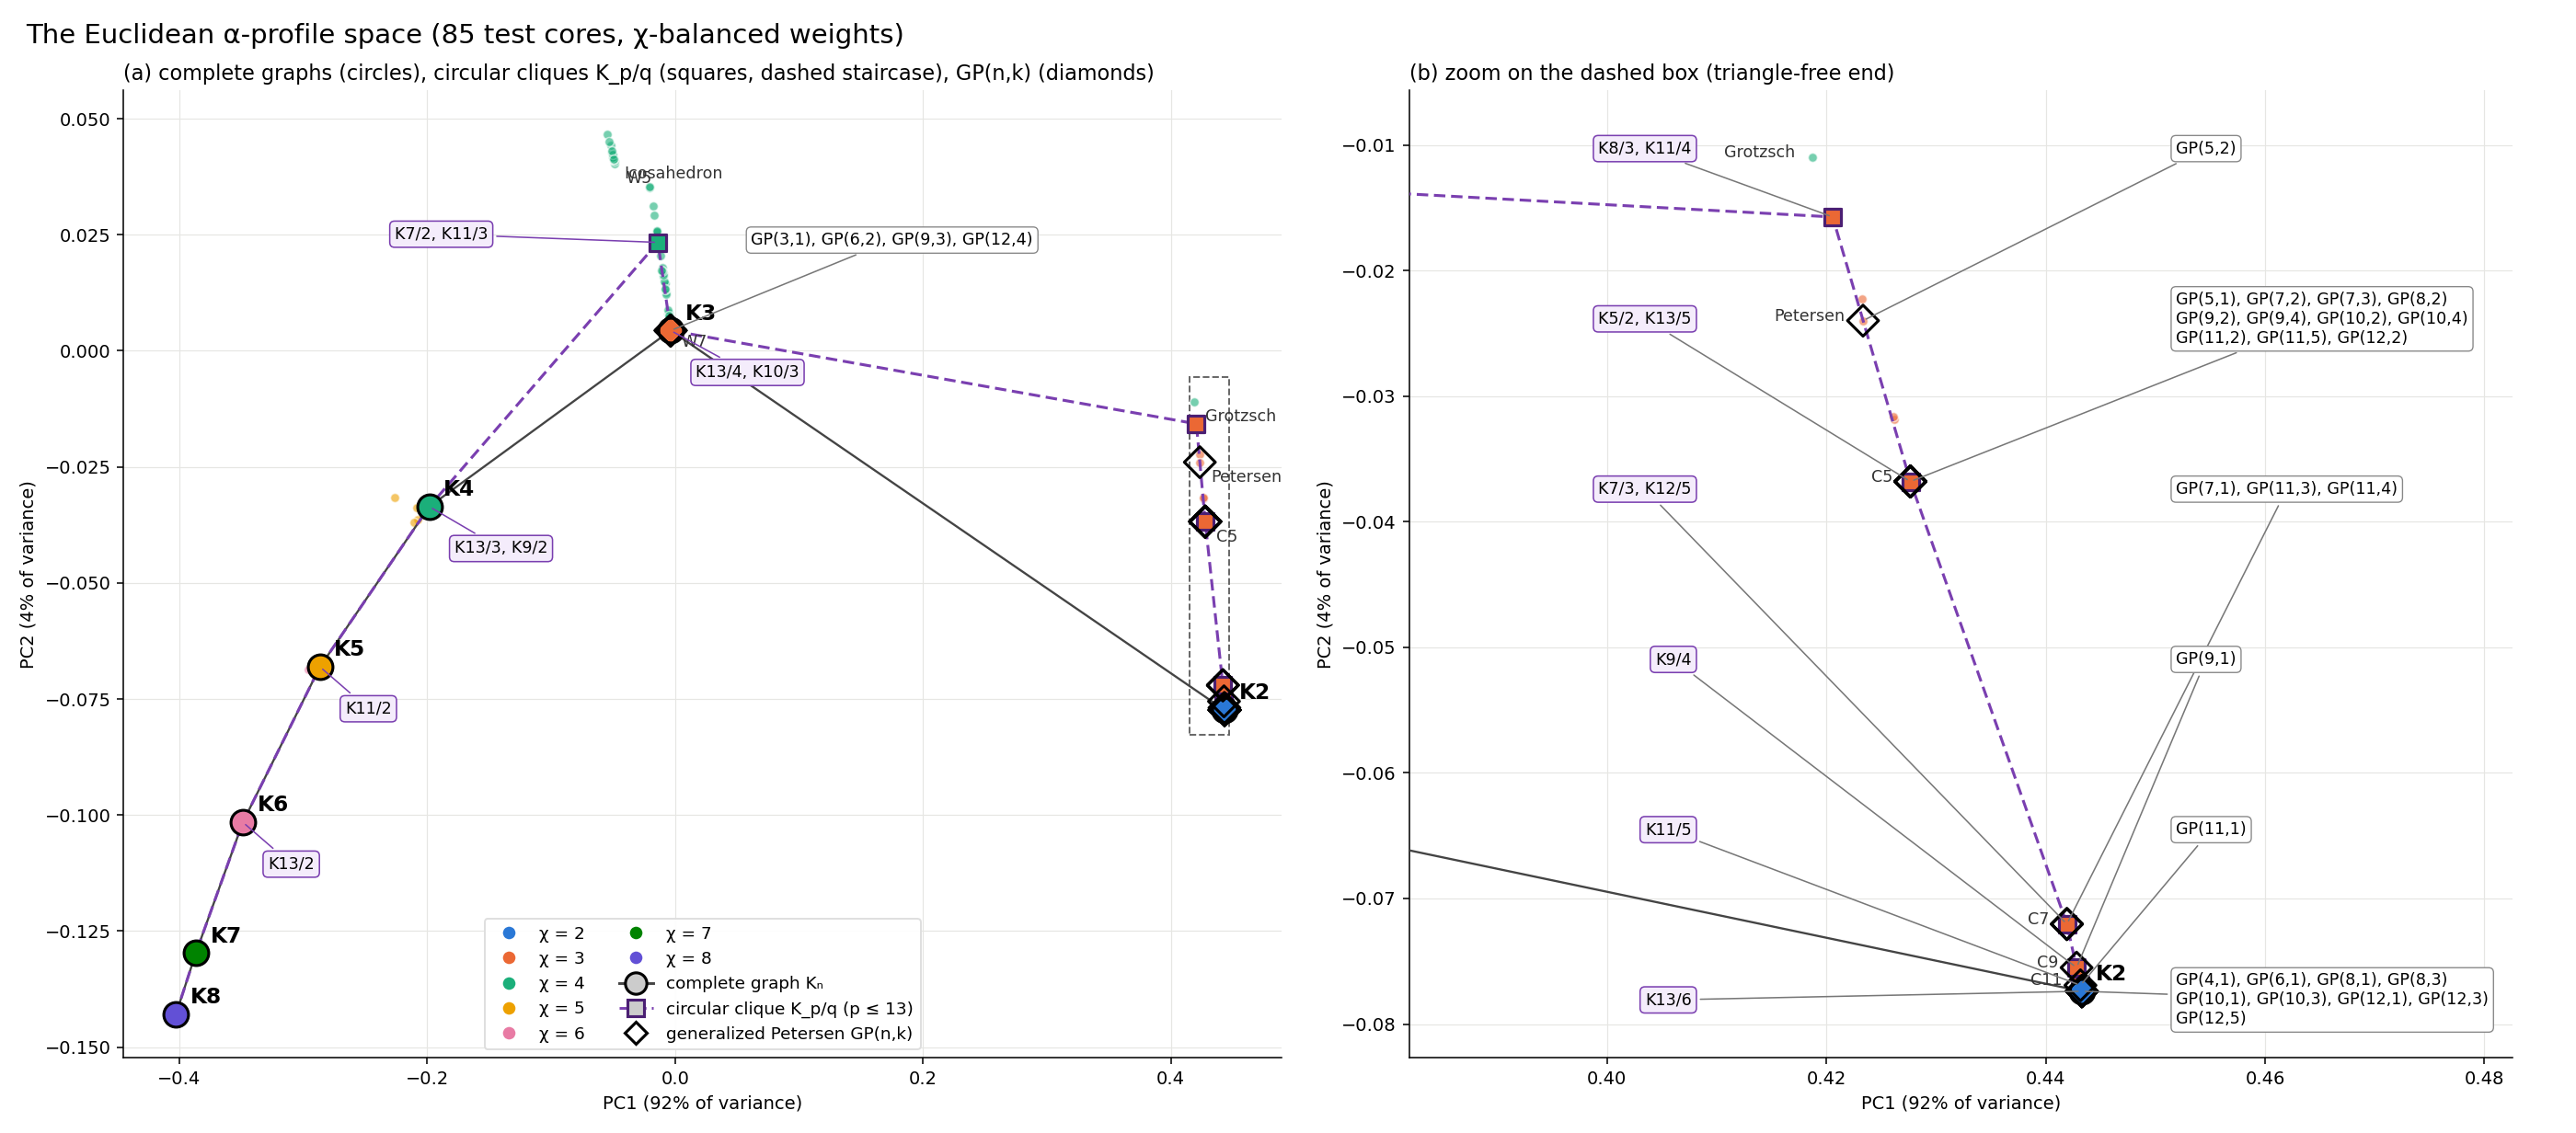
\includegraphics[width=\linewidth]{../figures/alpha_profile_pca.png}
\caption{The Euclidean profile space of the $85$ test cores ($\chi$-balanced
weights), first two principal components.  Large circles: complete graphs,
joined in order.  Squares joined by a dashed line: circular cliques
$K_{p/q}$, $p\le13$, in order of $p/q$.  Diamonds: generalized Petersen
graphs $GP(n,k)$, $n\le 12$.  Panel (b) zooms on the triangle-free end, where the odd cycles
accumulate at $K_2$.}
\label{fig:pca}
\end{figure}

\begin{figure}[ht]
\centering
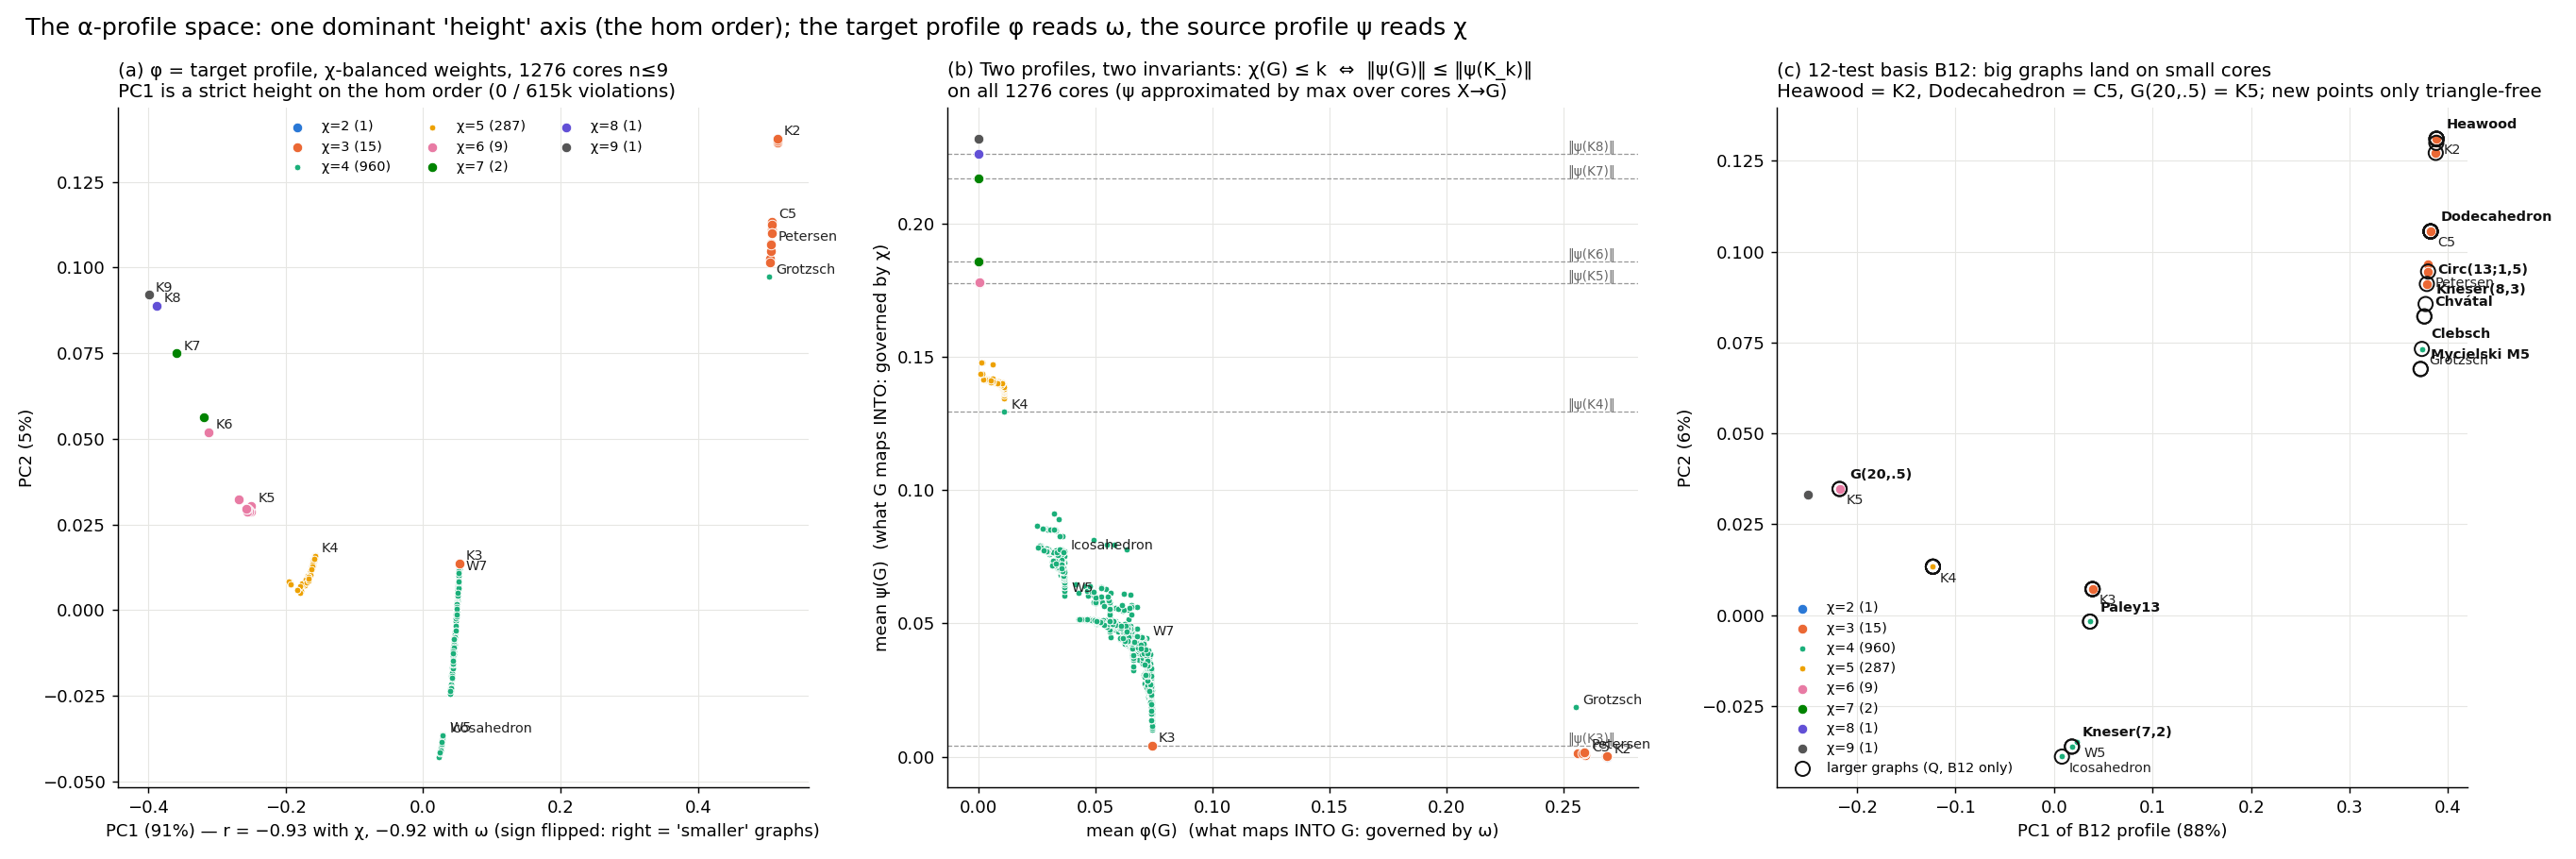
\includegraphics[width=\linewidth]{../figures/R_final.png}
\caption{(a) The $1276$ cores on at most $9$ vertices; the first principal
component is a strict height on the homomorphism order.
(b) Mean of $\varphi$ (what maps into $G$, governed by $\omega$) against
mean of $\psi$ (where $G$ maps, governed by $\chi$); here $\psi$ is
approximated by the maximum of $|X,T|/|E(X)|$ over cores $X\to G$ in the
data, which includes $X=G$.  (c) Larger graphs on a $12$-test basis land on
small cores; only triangle-free graphs of larger chromatic number give new
points.}
\label{fig:final}
\end{figure}

\paragraph{Circular cliques.}
We also computed the profiles of all $24$ circular cliques $K_{p/q}$ with
$p\le13$ and $2\le p/q\le8$.  Thirteen of them are themselves test graphs
($K_2,\dots,K_8$, $C_5$, $C_7$, $C_9$, $C_{11}$, $K_{7/2}$, $K_{8/3}$).
Each of the other eleven lands exactly on the point of the largest circular
clique below it whose numerator is at most $8$.  For example, $K_{13/6}$ lands on
$K_2$, $K_{12/5}$ on $C_7=K_{7/3}$, $K_{13/5}$ on $C_5$, $K_{11/4}$ on
$K_{8/3}$, $K_{10/3}$ and $K_{13/4}$ on $K_3$, $K_{11/3}$ on $K_{7/2}$, and
$K_{9/2}$ on $K_4$.  This is the staircase of
Proposition~\ref{prop:circular}, with an even coarser resolution than the
largest test ($12$ vertices) guarantees.  In particular, $K_{10/3}$ has
chromatic number $4$ but the same profile as $K_3$.

\paragraph{Separating families.}
On the $1276$ cores, every test family that separates all homomorphism
classes has at least $253$ members; a greedy search finds one with $311$.
The reason is structural.  Suppose $H\to G$, and $G-e\to H$ for every edge
$e$ of $G$ (a \emph{critical cover}).  Then a test $T$ separates $G$ from
$H$ only if every optimal map $T\to G$ uses every edge of $G$, which in
practice forces $T\leftrightarrow G$.  Of the $253$ forced pairs, $251$
are critical covers.  Adding the source-side coordinates $\psi_H$ removes
this obstruction.

% ---------------------------------------------------------------------------
\section{Open questions}

\begin{question}[Size of a separating family]
Let $\sigma(n)$ be the least size of a family $\mathfrak F$ such that
$\varphi$ restricted to $\mathfrak F$ separates all cores on at most $n$
vertices.  We know $253\le\sigma(9)\le311$.  Is $\sigma(n)$ comparable to
the number of cores on $n$ vertices?  Which cores are forced?
\end{question}

\begin{question}[Closure of the profile space]
The image of $\varphi$ is not closed: $\varphi(K_n)\to0$, and the Mycielski
chain converges to a point that is not the profile of a finite graph.  Is
the closure of $\{\varphi(G)\}$ in the product topology exactly the set of
profiles of countable graphs?  Is the space of homomorphism classes totally
bounded under $E_\infty$?
\end{question}

\begin{question}[Unweighted source-side profile]
Is $\sup_{X\to G}|X,T|/|E(X)|=\psi_T(G)$ for all $G$ and $T$, with the
supremum over simple graphs $X$?  Equality holds when $G$ is
edge-transitive.
\end{question}

\begin{question}[Is $d^*$ quasi-Euclidean?]
On cores with at most $9$ vertices, $d^*$ differs from $|\Delta\chi|$ by
at most $3$, yet $d^*\ge|\Delta\chi_f|$ suggests unbounded layers in
general.  Does $d^*$ admit a bi-Lipschitz embedding into $\ell^2$, or into
the profile space?
\end{question}

\section*{Acknowledgement of method}
The computations and parts of the arguments were developed with the help
of AI agents.  Propositions marked with citations are known; the remaining
statements have been checked on the data described above and should be
read as drafts until independently verified.

\begin{thebibliography}{99}

\bibitem{dgr2018}
H.~Dell, M.~Grohe and G.~Rattan,
``Lov\'asz meets Weisfeiler and Leman,''
in \textit{ICALP 2018}, LIPIcs vol.~107, pp.~40:1--40:14, 2018.

\bibitem{efjt2015}
R.~Engstr\"om, T.~F\"arnqvist, P.~Jonsson and J.~Thapper,
``An approximability-related parameter on graphs -- properties and
applications,''
\textit{Discrete Mathematics \& Theoretical Computer Science},
vol.~17, no.~1, pp.~33--66, 2015.

\bibitem{erdos1959}
P.~Erd\H{o}s,
``Graph theory and probability,''
\textit{Canadian Journal of Mathematics}, vol.~11, pp.~34--38, 1959.

\bibitem{fjt2009}
T.~F\"arnqvist, P.~Jonsson and J.~Thapper,
``Approximability distance in the space of $H$-colourability problems,''
in \textit{CSR 2009}, LNCS vol.~5675, pp.~92--104, 2009.
arXiv:0802.0423.

\bibitem{foucaud2019}
F.~Foucaud, H.~Hocquard, D.~Lajou, V.~Mitsou and T.~Pierron,
``Parameterized complexity of edge-coloured and signed graph homomorphism
problems,''
in \textit{IPEC 2019}, LIPIcs vol.~148, pp.~15:1--15:16, 2019.

\bibitem{hell2004}
P.~Hell and J.~Ne\v{s}et\v{r}il,
\textit{Graphs and Homomorphisms},
Oxford University Press, 2004.

\bibitem{khoshkha2005}
K.~Khoshkha,
\textit{Nonhomomorphism Factors},
M.Sc.\ thesis, Sharif University of Technology, 2005.

\bibitem{lrs2006}
M.~Langberg, Y.~Rabani and C.~Swamy,
``Approximation algorithms for graph homomorphism problems,''
in \textit{APPROX 2006}, LNCS vol.~4110, pp.~176--187, 2006.

\bibitem{lovasz1967}
L.~Lov\'asz,
``Operations with structures,''
\textit{Acta Mathematica Academiae Scientiarum Hungaricae}, vol.~18,
pp.~321--328, 1967.

\bibitem{vince1988}
A.~Vince,
``Star chromatic number,''
\textit{Journal of Graph Theory}, vol.~12, no.~4, pp.~551--559, 1988.

\bibitem{zhu2001}
X.~Zhu,
``Circular chromatic number: a survey,''
\textit{Discrete Mathematics}, vol.~229, pp.~371--410, 2001.

\bibitem{samal2015}
R.~\v{S}\'amal,
``Cubical coloring -- fractional covering by cuts and semidefinite
programming,''
\textit{Discrete Mathematics \& Theoretical Computer Science},
vol.~17, no.~2, 2015.

\bibitem{shitov2019}
Y.~Shitov,
``Counterexamples to Hedetniemi's conjecture,''
\textit{Annals of Mathematics}, vol.~190, no.~2, pp.~663--667, 2019.

\end{thebibliography}

\end{document}
